\documentclass[10pt]{article}
\usepackage[utf8]{inputenc}
\usepackage[english]{babel}

\usepackage[T1]{fontenc}
\usepackage{amsmath}
\usepackage{graphicx}
\usepackage{longtable}
\usepackage{algpseudocode}
\usepackage{algorithm}
\usepackage{tikz}
\usetikzlibrary{arrows}
\begin{document}
\title{\textbf{Smart Plant Monitoring System}}
\author{
\quad Sreeram Sadasivam \quad Vishwanath Vadhri \quad Christoph Peusens\\
\quad Supradha Ramesh \quad Mallikarjun Nutti\\
FB 20 Informatik\\
Technische Universität Darmstadt\\
\emph{\{sreeram.sadasivam,viswanath.vadhri,christoph.peusens,}\\
\emph{supradha.ramesh,mallikarjun.nuti\}@stud.tu-darmstadt.de}\\
\date{}
}
\maketitle
\textbf{\abstractname{
\emph {\textbf{\\
%ADD the abstract here...
Plant monitoring is seen as one of the most important tasks in any farming or
agriculture based environment. 
With the inception of Ambient Intelligent
systems, there have been a rise in ambient intelligent based devices - Smart Homes\cite{ref001} and other similar technologies involving RFID has evolved over the past few years\cite{ref002}. 
Integration of such an ambient intelligent system with plant monitoring makes farming easier. 
In this paper, we discuss about the implementation of a smart plant monitoring system which makes use of the concept ambient intelligence with the use of .Net Gadgeteer which, proactively handles the plant monitoring system. 
The given implementation works along with a cloud based server and a mobile based device (ideally Android/iOS device) which helps the user to control and see the status of the plant which is being monitored by the hardware device. 
The given circuitry detects changes in the moisture, temperature and light conditions in and around the plant, and performs a machine based curation on the plant by providing necessary irrigation and illumination for the plant. 
Machine curation is also integrated with active weather forecasting systems which are deployed in the cloud based server using which advanced machine curation is performed. 
For user based curation, the Android device provides user an option to override a machine curated operation. %conclusion statement to be added...
}}}}

\section*{Motivation}

%Add the motivation part here...
The most important factors for the quality and productivity of plant growth are temperature, humidity, light and the level of the carbon dioxide. 
Continuous monitoring of these environmental variables gives information to the grower to better understand, how each factor affects growth and how to manage maximal growth of plants. 
Climate control and monitoring of the plant is one of important aspects in agriculture. 
The aspects we are presenting resembles the concept of precision agriculture, this is the trend of farming presented in recent years for commercial and research agriculture\cite{ref005}. 
In the precision agriculture framework the focus is mainly on understanding the environment through the interpretation of a wide variety of data coming from GPS systems, satellite imaging, and in-field sensors.Cypress is one of top semiconductor company in the world. Currently they have envisioned the scope by moving towards Internet of Things,with the major focus on ``Internet of plants''.  
The main motivation of the project is for the user to monitor the plants or cultivation to get enough resources such as light and water without the user need to be present at the plants or cultivation area, and also could manipulate the resources provided to the plants depending on the climate of the plant's location(Example : if there is enough rain or moisture for the day, the sensor in the soil would detect accordingly for the operation to begin and intimate the user).
This could help user not only to give the resources to the plants everyday without much manual effort also helps the constant and healthy growth of a plant.


\section*{Related Works}

%Add some related work here...



Mancuso et all~\cite{ref003}, has done a similar research work in a tomato greenhouse in the South of Italy. 
They are using Sensicast devices for the air temperature, relativity humidity and soil temperature measurements with wireless sensor network. 
They have also developed a Web-based plant monitoring application. 
Greenhouse grower can read the measurements over the Internet, and an alarm will be sent to his mobile phone by SMS or GPRS if some measurement variable changes rapidly. 
Bridge node gathers data from other sensor nodes, which transmit the measurements of temperature and relative humidity in one minute intervals. 

Teemu Ahonen et al~\cite{ref004}, has done the research in Martens Greenhouse Research Center’s greenhouse in the Närpiö town in Western Finland, they had integrated three commercial sensors with Sensinode’s sensor platform to measure four environmental key variables in greenhouse control.
The system feasibility was verified in a simple star topology setup in a tomato greenhouse.
The sensors used were SHT75 humidity/temperature sensor and TSL262R light irradiance sensor, and Figaro’s TGS4161 CO2 sensor used. 
Application of the concept in the greenhouse: temperature, luminosity and humidity sensors measured climate variables and communicated directly with the gateway node. 
The gateway node acted as a coordinator and received the measured data from the sensor nodes. 
The maximal communication range, 15 meters was figured out in individual test where the distance between the coordinator and the sensor node inside the greenhouse dense flora was increased,the reliable communication range fell to one third in the greenhouse's dense flora. 

\section*{Design}

%Add design here...
The proposed system consists of two curation systems. 
The first one being the \emph{machine based curation} and other being the \emph{user based curation}. 
These curative systems are in place to provide a smart and involuntary feedback to the given environment. 
The former is more of predictive system devised on a hardware whereas, the latter is for the user to actively handle the response provided by hardware. 
The curation handled by the device are based on the sensor information it receives from its end points(\emph{sensory hardware units}), such a curation is called as \emph{``Direct Machine Based Curation''}. 
There is also a hybrid machine based curation provided by the device and the cloud server which relies on the Weather Forecast information with the collects sensor values from the endpoints, such a curation can be called as \emph{``Advanced Machine Based Curation''}. 
If the user wants to take over the system then, it becomes more of a \emph{``User Based Curation''}. 
On top of all, the proposed system design is a pub-sub system. 
The Monitoring hardware is the publisher and Mobile based devices are subscribers. 
The cloud based server act as \emph{``brokers''}. 

\subsection*{Basic Interaction}

Primarily the interaction between the monitoring device and the user enabled mobile device happens as a publisher-subscriber system. 
This interaction is brokered by the cloud based server with monitoring hardware and the mobile device as the publisher and subscriber respectively. 
The Cloud Based server - ``Parse''~\footnote{See www.parse.com/docs} provides core functionalities. 
This server not only gives a hand for machine based curation but also, in providing various push based services to the Mobile Device(Android/iOS/Windows).
The monitoring hardware used for this system is .Net Gadgeteer~\footnote{See www.netmf.com/gadgeteer/}. 
Before any curation to work the device must initially register to the cloud server by their respective device tokens thereby, the broker service can later on perform push services. 
For handling the registration operation, the server have provided two different registration APIs --- one for the Android/iOS/Windows device using which mobile device can register itself and also subscribe to a particular monitoring device.
And the other for the Monitoring hardware device in order for registering to server with its Geo-Location. 
Once the registration is successful the device and user can perform curations.
The mobile application deployed in the mobile device informs the user about the device status and weather status in the location of subscribed monitoring device using which user can perform the curation of the system(\emph{Ref:Table~\ref{tab:API_TAB}}).\\ 
\pagebreak
\begin{center}
\begin{longtable}{| p{.35\textwidth}| p{.20\textwidth}| p{.20\textwidth} | p{.40\textwidth} |}
%\begin{tabular}{| l | l | l |p{4cm} |}
   \hline
   \textbf{API} & \textbf{Type} & \textbf{Target} & \textbf{Summary} \\ \hline

   \emph{register} & Registration &.Net Gadgeteer & Registers the  Device ID of Gadgeteer to the server and also provides the Geo Location to the server.
   \\ \hline


   \emph{extDeviceRegister} & Registration & Android/iOS & Registers the mobile device to the server and subscribes to a gadgeteer device by providing the Device ID of Gadgeteer as one of the inputs.
   \\ \hline

   \emph{deviceStatus} & Device & Android/iOS & Provides the status such as water, light modules of monitoring device to which the mobile device has subscribed to.
   \\ \hline
   
   \emph{updateDeviceStatus} & Device & .Net Gadgeteer & Updates the device status of the monitoring hardware device in the server. When such a modification happens an event is triggered to all the subscribed mobile devices(a push based service). 
   \\ \hline

	\emph{manualOverride} & Device & Android/iOS & Modifies the device status of the monitoring hardware device in the server. When such a modification happens an event is triggered to the subscribed gadgeteer device(a poll based service). 
   \\ \hline

	\emph{pollForDevice} & Device & .NetGadgeteer & Polling mechanism implemented for monitoring hardware thereby, the hardware can poll for events created by mobile interfaced user.
   \\ 
   \hline   
 
	\emph{weatherStatusForDevice} & Weather & Android/iOS & Provides the weather condition in the location of monitoring device to which the mobile device has subscribed to.
   \\ \hline      
\pagebreak
   \hline
	\emph{weatherForecastForDevice} & Weather & Both & Provides the weather forecast to the gadgeteer for the timeline of closest 3 hour time slot. In case of mobile device, it provides an overall forecast which includes for the next 24 hrs from the current time. 
   \\ \hline      

\caption{API Table} % needs to go inside longtable environment
\label{tab:API_TAB}

\end{longtable}
%\end{tabular} 
\end{center}

\subsection*{Machine Based Curation}

 As said stated in main section, machine based curation works in two modes --- \emph{Direct} and \emph{Advanced}. 
In case of \emph{``Direct''}, the cloud server acts as a \emph{``broker''} between the Mobile device and the Monitoring Hardware. 
Whereas in case of \emph{``Advanced''}, it is more of a hybrid model where both weather forecast information provided by the server and sensor data collected by the device are considered before performing an event.

\subsubsection*{Direct Mode}

The sensor nodes detects the changes in the environment around the monitoring plant such as - light, moisture. 
Based on these values the monitoring device will curate the events to be handled in the system. 
The curation is very straight-forward due to which it is called as \emph{``Direct''}. 
The monitoring hardware is integrated with moisture and light sensors which can help in providing valid curations to the system. 
Moisture sensors readings are compared with the threshold values set in the monitoring hardware and necessary actions are performed. 
If the moisture reading is low and, as per the plant configuration the watering for the plant is required then, the plant will get watered accordingly.
The same happens with light illumination on the plant, the light sensor deployed with the Gadgeteer detects the light change and accordingly turns ON the artificial light provided.
The direct mode completely relies on the sensor nodes and gadgeteer device.

\subsubsection*{Advanced Mode}

Hybrid machine curation is based on predictive inputs provided by the server and the sensor inputs from the sensory nodes. 
For the implementation of such a mode, the system requires to get access of weather forecast of the location where the monitoring unit is present.
Such an implementation is handled by the \emph{weatherForecastForDevice} API provided by the server.
Such a service is invoked by the monitoring device only when it believes it has encountered a minimum threshold for its activity. 
For example, the monitoring device when it detects the reduction in moisture content in system and requires the \emph{``Direct''} mode to take over.
Instead of such a takeover the \emph{``Advanced''} mode of operation is initiated.
In this mode of operation, the device performs curation with the server as well. 
Thus making the system more of a hybrid model.
When the monitoring hardware decides to invoke the weather forecast API, it sends its current device time using which the server can send back the forecast time slot for the device.
The time slot mechanism is handled based on the time provided by the device.

\begin{algorithm}
\caption{Calculate Time Slot}          % give the algorithm a caption
\label{time_alg}      
\begin{algorithmic}
\\
\State $timedif \gets devtime - curtimeslot$
\If {$timedif \geq 0$}
    \State $timeslot\gets timedif/timeslotduration$
    \If {$timeslot \leq maxtimeslot$}
        \If {$weatherinfo[timeslot] \neq ``Rain''$ }
        		\State $isRain \gets false$
    		\Else
    			\State $isRain \gets true$
    		\EndIf
    \Else
    		\State $return \gets ``Invalid Device time''$
    \EndIf
\Else
    \State $return \gets ``Use Previous Forecast Data''$
\EndIf
\State $return \gets isRain$
\end{algorithmic}
\end{algorithm} 

\begin{figure} [!ht]
\centering
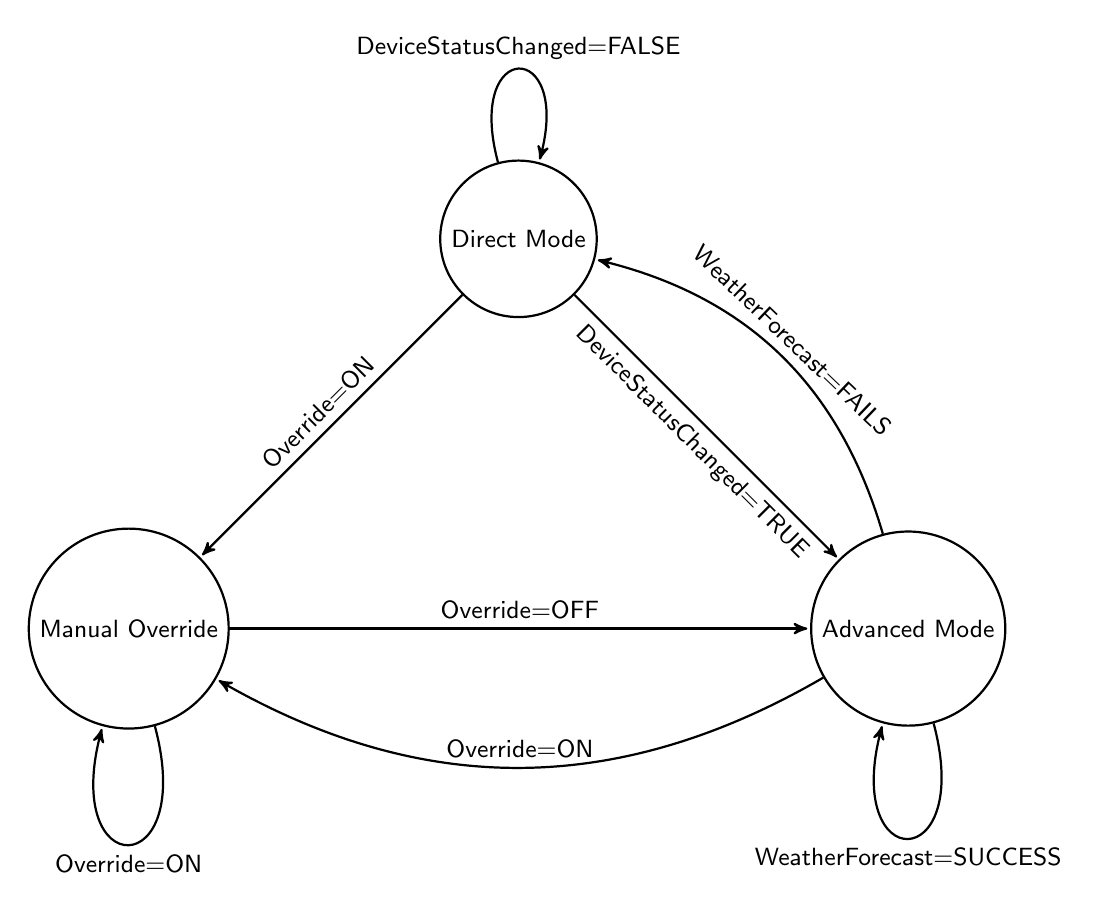
\begin{tikzpicture}[->,>=stealth',shorten >=1pt,auto,node distance=7cm,
                    thick,main node/.style={circle,draw,font=\sffamily\small}]

  \node[main node] (1) {Direct Mode};
  \node[main node] (2) [below left of=1] {Manual Override};
  \node[main node] (3) [below right of=1] {Advanced Mode};

  \path[every node/.style={font=\sffamily\small}]
    (1) edge [loop above] node {DeviceStatusChanged=FALSE} (1) 
	    edge node [sloped,above] {Override=ON} (2)
        edge node [sloped,below] {DeviceStatusChanged=TRUE} (3)
    (2) edge node [above] {Override=OFF} (3)
        edge [loop below] node {Override=ON} (2)
        %edge [loop left] node {0.4} (2)
    (3) edge [bend left] node [above] {Override=ON} (2)
        edge [bend right] node[sloped,above] {WeatherForecast=FAILS} (1)
        edge [loop below] node {WeatherForecast=SUCCESS} (3);
\end{tikzpicture}
\caption{State Diagram Of Mode Change-Overs}
\label{fig:ModeChangeOverStateDiagram}


\end{figure}


\subsection*{User Based Curation}

The user based curation is hand held by the user using the Android/iOS devices. 
The user can curate the device and weather statuses of the monitored device using his/her mobile device.
Using the data provided by the android application, the user can perform override functionalities (if required) by the user.
The standard APIs provided by the server can be used by the user's mobile application to handle the device and weather statuses.
The user can also invoke the weather forecast API which was provided for advanced machine curation.
The forecast API does not work the same way as for the gadgeteer. 
In case of invocation from the mobile device, the forecast API provides a generic weather forecast for the next 24 hrs. 
Using such an information the user can perform much more intelligent decisions.
User curation is handled by having the option for the user to perform manual override option from the Android device.
Since the current implementation of the Parse SDK does not support the Gadgeteer.
The system performs a polling service from monitoring hardware. 
The Gadgeteer polls the server to see if there is any new event waiting for the Gadgeteer to service upon.
If it finds the servicing, then it handles the change and performs a update device status API call to the server. 
Thereby, triggering a push to the user's mobile device.

\subsection*{Working with Modes}

The Gadgeteer initially sets itself in \emph{``Advanced''} mode and later on changes to \emph{``Direct''} mode based on the correctness of the forecast.
When the forecast fails the gadgeteer retracts itself to \emph{``Direct''} mode. 
For more info refer Algorithm~\ref{ModeChangeoverAlgo}. There is a switching between curations as well. For more info about switching curations and modes, refer to Fig~\ref{fig:ModeChangeOverStateDiagram}.

\begin{algorithm}
\caption{Mode Change Over}          % give the algorithm a caption
\label{ModeChangeoverAlgo}      
\begin{algorithmic}
\\
\State $mode \gets ``Advanced''$
\If {$forecast$ is $success$}
    \State $return \gets``No mode change needed''$
\Else
    \State $mode \gets ``Direct''$ until next time slot
\EndIf
\State $return \gets mode$
\end{algorithmic}
\end{algorithm} 

%\begin{tikzpicture}[shorten >=1pt,node distance=5cm,on grid,auto] 
%   \node[state,initial] (q_0)   {$Advanced Mode$}; 
%   \node[state] (q_1) [above right=of q_0] {$Direct Mode$}; 
%   \node[state] (q_2) [below right=of q_0] {$Manual Override Mode$}; 
%    \path[->] 
%    (q_0) edge  node {WeatherForecast = failed} (q_1)
%          edge  node {ManualOverride} (q_2)
%    (q_1) edge  node  {1} (q_2)
%          edge  node {0} (q_0)
%    (q_2) edge  node {0} (q_0) 
%          edge  node {1} (q_2);
%\end{tikzpicture}
\pagebreak
\section*{Evaluation}

%Add evaluation here...
The proposed system encounters multiple change-over schemes with respect to the curation mechanism in place.\\

\begin{longtable}{p{1.0\textwidth}}%{p{10cm}}
\hline \\
\textbf{Scenario 1:} Notification given by hardware device to user(weather forecasting with the chance of rain)  \\
\hline    \\

The device set in advanced mode.\\
As mentioned in the design and basic interactions the hardware device and android device acts as the pub-sub system and the cloud- based server acts as the broker between both systems. The system works as follows:
\begin{itemize}
\item
The hardware device checks the moisture or humidity of the plant soil and if the threshold value( when the plant needs water ), the weather forecast has been invoked to check if in next 1 hour if it would rain or not.
\item
If there is chance of rain, the event for watering the plants has not been triggered.
\end{itemize}\\

\pagebreak
\hline \\
\textbf{Scenario 2:} Notification given by hardware device to user(weather forecasting with no chance of rain)\\
\hline
\\
The device set in advanced mode.
As mentioned in the design and basic interactions the hardware device and android device acts as the pub-sub system and the cloud- based server acts as the broker between both systems.\\ The system works as follows:
\begin{itemize}
\item The hardware device checks the moisture or humidity of the plant soil and if the threshold value( when the plant needs water ), the weather forecast has been invoked to check if in next 1 hour if it would rain or not.
\item If there is no chance of rain, it issues the event change to the user and starts watering the plants.
\item If the user doesn’t want the plants to be watered, he can override the event and stop from watering the plants.
\item Now after the manual override the device mode is set to manual mode. In manual mode( for certain time “X” period, only the manual override would be set.As to avoid continuous notification and working of the hardware.
\end{itemize}
\\
\hline \\
\textbf{Scenario 3:} Notification given by hardware device to user\\
\hline
\\
The device is set in advanced mode 
\begin{itemize}

\item If the weather forecast fails in both the above mentioned scenarios 1 and 2 , The device is set in direct mode, where the hardware device will take over event required resources the plant needs automatically.
\end{itemize}
\\
\hline
\\
\textbf{Scenario 4 :} Notification given by hardware device to user( light resource)\\
\hline 
\\
The device is set to advanced mode.
As mentioned in the design and basic interactions the hardware device and android device acts as the pub-sub system and the cloud- based server acts as the broker between both systems. \\The system works as follows:
\begin{itemize}
\item The hardware device checks the light threshold value and sends a notification to the user regarding its event for switching on the light.
\item If the user wants to override the event, he could manipulate it as mentioned above.
\end{itemize}\\ 
\hline \\
\pagebreak
\hline \\
\textbf{Scenario 5:} Notification given from user to hardware device\\
\hline\\
The device is set to manual mode.
As mentioned in the design and basic interactions the hardware device and android device acts as the pub-sub system and the cloud- based server acts as the broker between both systems.\\
 The system works as follows:
\begin{itemize}
\item The user manipulates the resources to his plant according to the convenience of user.
\item If the user is at different location from the location of the plant. the user can request for the (invoke) weather forecast of the plant location and according to the forecast the user can decide on what resources to be given to his/her plant.
\end{itemize}
\\
\hline
\end{longtable}


\section*{Conclusion and future outlook:}

The efficient automation on monitoring and control of the plants require new and revolutionary solutions. Wireless sensor networks can respond to requirement by offering an accurate and easily configurable monitoring system.In this work we are using the the moisture sensor and light sensor with which, we could efficiently monitor the basic resources of the plant .This is prototype of the monitoring and control system for plants.Unlike other automated systems which relies on automated data,our model is more “Intelligent” to utilize the resources according to the changes in weather conditions. Our model has the capability to integrate with any mobile platform, Since the broker service is running on a cloud based service it is scalable.

For future outlook, we could add certain functionality for making the system more smart by uploading the configuration of the plant at the time of set upset, through the hardware device interface.functionalities like scheduled manual override can be added.camera monitoring , live streaming of the plant , we could use wowza streaming engine which uses RTSP and RTMP.

\section*{Acknowledgment}

The authors would like to thank Florian Müller of Tele-Kooperation(TK) from Informatik department of Technische Universität Darmstadt for providing the opportunity to work in the selected topic.


%Bibliography....
\begin{thebibliography}{1}

\bibitem{ref001}
Kidd, CoryD. et,al. \emph{``The Aware Home: A Living Laboratory for Ubiquitous Computing Research''}.\hskip 1em plus
  0.5em minus 0.4em\relax  Springer Berlin Heidelberg (1999).

\bibitem{ref002}
Antonio J. Jara, Miguel A. Zamora, and Antonio F. Skarmeta.  \emph{``An internet of things---based personal device for diabetes therapy management in ambient assisted living (AAL).''}.\hskip 1em plus
  0.5em minus 0.4em\relax Personal Ubiquitous Comput. 15, 4 (April 2011), 431-440.  
  
\bibitem{ref003}
M. Mancuso and F. Bustaffa, \emph{``TA Wireless Sensors Network for Monitoring Environmental Variables in a Tomato Greenhouse''}.

\bibitem{ref004}
Teemu Ahonen, Reino Virrankoski and Mohammed Elmusrati , \emph{``Greenhouse Monitoring with Wireless Sensor Network''}.\hskip 1em plus
  0.5em minus 0.4em\relax University of Vaasa

\bibitem{ref005}
TongKe, Fan. \emph{``Smart Agriculture Based on Cloud Computing and IOT.''}\hskip 1em plus
  0.5em minus 0.4em\relax Journal of Convergence Information Technology 8.2 (2013).

\bibitem{ref006}
Zhang, Xiang Wen, Ran Chen, and Chun Wang. \emph{``Design for Smart Monitoring and Control System of Wind Power Plants.''}\hskip 1em plus
  0.5em minus 0.4em\relax Advanced Materials Research. Vol. 846. 2014.
  
\bibitem{ref007}
Chen, Joy Iong Zong, Yuan-Chen Chen, and Shien-Dou Chung. \emph{``Implementation of a Greenhouse Crop Remote Monitoring System with IOT Technology.''}
  
\end{thebibliography}
\end{document}
